
\ChapterWithSubtitle{Evaporation of water by boiling}{water water every where}
%\chapter{Heating by Radiation}

%%%%%%%%%%%%%%%%%%%%%%%%%%%%%%%%%%%%%%%%%%%%%
\section*{Equipment List}

\begin{multicols}{2}   % change 2 -> 3 for three columns
\begin{equipment}
\item Ruler
\item Stopwatch
\item Digital Thermometer
\item Apron
\item 250 mL beaker
\item mini scale
\item hot plate
\item tongs
\item safety goggles
\end{equipment}
\end{multicols}


%%%%%%%%%%%%%%%%%%%%%%%%%%%%%%%%%%%%%%%%%%%%%
\section{Introduction and Definitions}

Today we begin a serious study of water.  Water is of course directly important to life on Earth --- it played a key role in the evolution of life from microscopic organisms to the zoo that currently populates the planet (including ourselves!), and our bodies are more than half water by weight --- but it is also a key factor in controlling the Earth's climate.  Over the past week we showed that water ($\text{H}_2\text{O}$) is an asymmetric molecule with a permanent electric dipole moment and, more importantly, it has a {\em changing} dipole moment when vibrating or rotating.  We discussed the implications of this for the greenhouse effect.  Sketch  a 3D picture of the water molecule (recall that it is {\em tetrahedral} if you include the ``lone pairs'' on the oxygen atom) and discuss very briefly the implications of its shape and its electric dipole moment on our climate.

\answerspace

\noindent This week and next we will discuss a second important way that water influences our climate --- and contributes to the full answer of the question that drives the first half of this course: {\em What is the expected equilibrium temperature\footnote{Recall our prior calculations: (i) the balance of the Sun's incoming radiation flux with the Earth's outgoing infrared radiation, $F_\text{sun} = F_\text{earth} (T)$, led to an equilibrium temperature of about $-15\degree$C; (ii) assuming an atmosphere that blocks all infrared light from the Earth's surface (and then re-emits it both out to space and back down to the surface) we found an equilibrium temperature of about $+30\degree$C. Neither of these is yet correct, since our average surface temperature is about $+15\degree$C.} of the Earth?}  The mechanism of this influence is essentially the same one that our body uses to cool us when exercising: {\em perspiration}.  Say a few words about how perspiration works for the human body --- and maybe also note some conditions that prevent it from working, or decrease its efficacy --- and try to make an energy flow diagram demonstrating why the internal energy of a body decreases during perspiration.

\answerspace[3cm]

\noindent Check in with your neighbors and instructor regarding the answers to the questions in this section.

%%%%%%%%%%%%%%%%%%%%%%%%%%%%%%%%%%%%%%%%%%%%%
\subsection{Phase transitions and water}

On one of the following pages you will find what is called a {\bf phase diagram} for water.  A fixed volume/amount of water under various temperature and pressure conditions will take different forms: solid, liquid, or gas/vapor.  Note that the ``pressure'' axis has a logarithmic scale to show a wide range of values.  Let's explore this diagram a little bit. First, from your own personal experience, describe these three phases of water very briefly.

\answerspace[2cm]

\noindent Temperature should be familiar to you. Remind yourself and your neighbors what a few familiar values in Fahrenheit correspond to in the Celsius and Kelvin scales.

\answerspace[2cm]

\noindent Pressure might be less intuitively familiar.  You may have personally experienced pressure when diving to the bottom of a swimming pool. If you're not familiar with the effect, find someone in your group who has experienced it, and ask them to describe how it felt.  This experience is due to an {\em increase} in pressure --- on top of the normal {\bf atmospheric pressure} value of our surrounding air\footnote{Atmospheric pressure is also the value of the water pressure at its surface.} ---  due to the {\em weight of water} above you.  Now, knowing that the pressure {\em outside} of our atmosphere is zero (space is a ``vacuum''), and making an analogy to the swimming pool, describe why there is a non-zero atmospheric pressure at the surface of the Earth.

\answerspace

\noindent Look up the value of our atmospheric pressure (pressure is force per area, and the standard unit is the {\em Pascal}, with  $\unit{1}{\pascal} = \unit{1}{\newton/\meter^2}$).  Also look up how much its value varies over a few days (pressure is a standard parameter reported with the weather).  State these values below and then show the approximate atmospheric pressure value on the phase diagram using a ruler to make a horizontal line across the whole figure.

\answerspace[2cm]

\noindent Now consider the process of water {\bf freezing}.  Along the line of atmospheric pressure, draw a point {\bf A} that sits in the liquid water section.  Note its temperature, $T_A$.  Then draw an arrow along the line of atmospheric pressure toward solid water.  Which direction are you going (in temperature) and at which temperature --- call it $T_f$, the temperature of freezing --- does the phase change from liquid to solid?  Also: how much would your answer for $T_f$  have changed if the atmospheric pressure line was different (e.g., ten times bigger or smaller).

\answerspace[3cm]

\noindent Today we will focus on the process of {\bf vaporization} (or, {\em evaporation}, or {\em boiling}). Go back to your $T_A$ point and draw an arrow toward vapor.  Which direction are you going (in temperature) and at which temperature --- call it $T_v$, the temperature of vaporization --- does the phase change from liquid to vapor?  

\answerspace[1.2cm]

\noindent How much would your answer for $T_v$  have changed if the atmospheric pressure line was different (e.g., ten times bigger or smaller)?  Is this the same or different than what you found for the liquid-solid transition?



%%%%%%%%%%%%%%%%%%%%%%%%%%%%%%%%%%%%%%%%%%%%%
%%%%%%%%%%%%         Phase diagram for water         %%%%%%%%%%%%%%%
%%%%%%%%%%%%%%%%%%%%%%%%%%%%%%%%%%%%%%%%%%%%%
\newpage

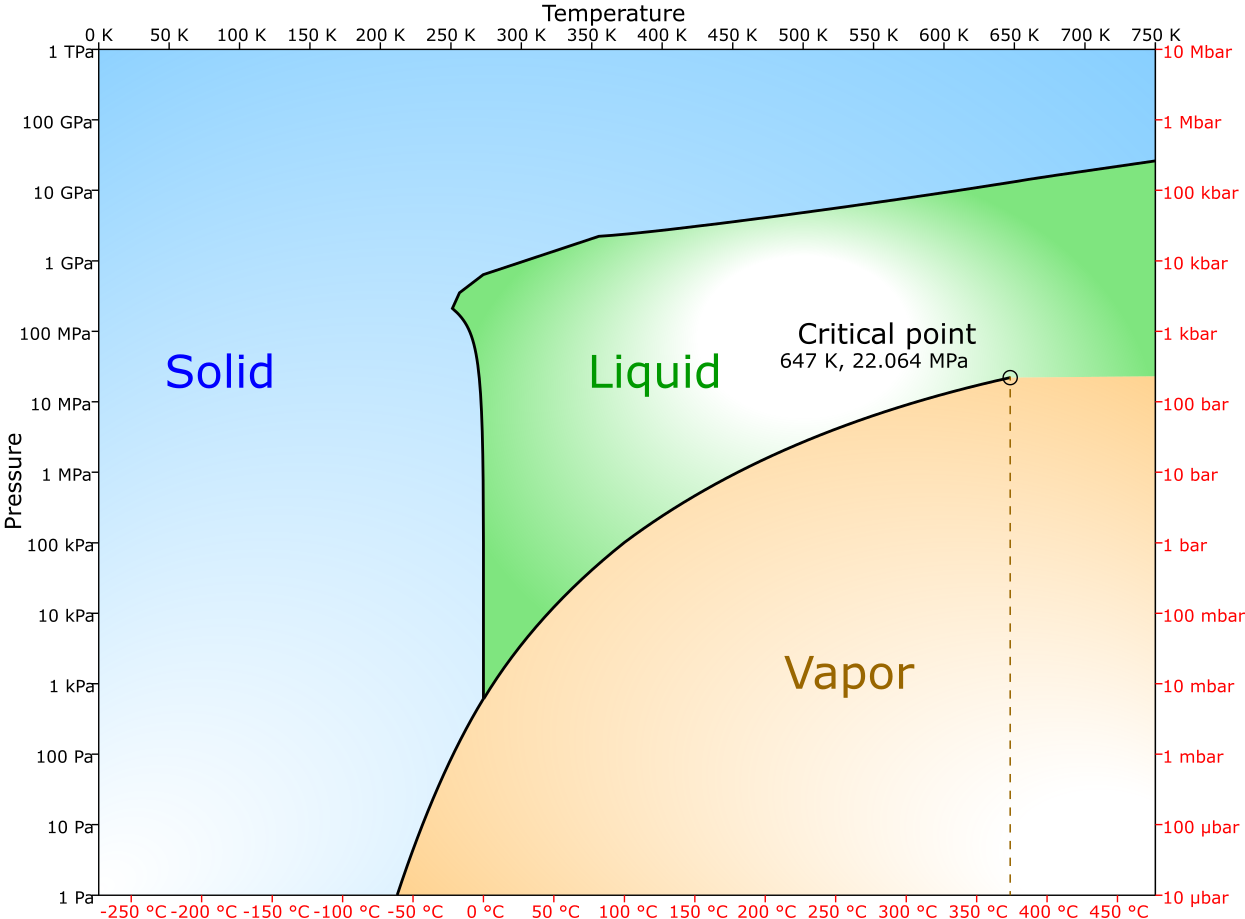
\includegraphics[width=\textheight, angle=90]{images/07_phase-diagram-of-water-simplified_wikimedia-Cmglee_edited.png}


\newpage
%%%%%%%%%%%%%%%%%%%%%%%%%%%%%%%%%%%%%%%%%%%%%
%%%%%%%%%%%%%%%%%%%%%%%%%%%%%%%%%%%%%%%%%%%%%


%%%%%%%%%%%%%%%%%%%%%%%%%%%%%%%%%%%%%%%%%%%%%
\section{Experiments and Analysis}

{\bf \underline{Safety Note}:} We will boil water on the hotplate today, and will will repeatedly transfer it back and forth from the hotplate to the scale to measure mass. You should take great care in this procedure, i.e.,  focus on tightly grasping the tongs around the beaker, just below the rim, during each transfer. Do not get distracted by other tasks or your partners while doing so. As noted in the prcedure below, it is recommended that you alternate your temperature and mass measurements so that you don't try to do two things at once.  You should also be wearing long pants and closed shoes so that if boiling water were to spill you would be partially protected. But everyone should be alert and aware during the boiling procedure as well.  You will wear safety googles for the boiling procedure to protect your eyes (these can be worn over glasses).

\subsection{Boiling water!}

We will take data on the process of vaporization using a hotplate and about 200~mL of water in a 250~mL beaker.  Our goal is to monitor both temperature and mass over time and then use the rates (of temperature increase before the ``boiling point'', and mass decrease after) to determine the so-called latent heat of vaporization, $L_v$.

\vspace{0.5cm}

\noindent {\bf Read through the entire procedure before beginning.  Listen to tips on safety and effectiveness from your instructor.}

\vspace{0.5cm}



\noindent {\bf Procedure:} Using your own paper (and/or a Google sheets spreadsheet) to write down observations, keep a data table, and make calculations from equations --- take the following basic steps.
	%
	\begin{itemize}
	\item I would recommend a google sheets spreadsheet with these columns: [minutes, seconds, t~(s), Mtot (g) , T(C)].  Then in the first two columns you can just record the time on your stopwatch (e.g., 3:53 is 3 in the minutes and 53 in the seconds column).  Later you will calculate the ``t(s)'' column values using an excel formula like ``\verb|=b2*60 + c2|''. 
	\item Place your empty beaker together with your digital thermometer on the mini scale and measure their mass together.  Record this value so that you can subtract it off from your mass measurements in the end.
	\item Put about 200~mL of tap water in your beaker.  With the thermometer inside, place it on your scale to get an initial mass measurement (your mass measurements will always include the beaker and thermometer).
	\item Start your stopwatch.
	\item Turn on your hotplate to $450\degree$C and place your 250~mL beaker of water (with thermometer) on its center.
	\item Use the blue labjack to arrange your miniscale so that it is immediately to the side of your hotplate and at the same level, so that transfers back and forth will be easier.
	\item Start taking data of temperature and mass, at approximately 1 minute intervals for each. I would recommend alternating every thirty seconds between mass and temperature, so that you don't have to take the temperature while measuring the mass.  It is perfectly fine for the temperature and mass values to be recorded at different times.
	\item For mass measurements, carefully grip the beaker with the tongs and carry it over to the scale.  Relase it and have a partner record the mass measurement.  Then grip it tightly again and bring it back to the hotplate.  This should take about 10 seconds out of every minute of warming.  Always be careful, but don't remove the beaker from the hot plate for very long.
	\item For temperature measurements, raise the thermometer above the bottom of the beaker and use it to stir for a few seconds before recording a measurement.
	\item Take data until the temperature reaches the boiling point, and then continue for at least 10 more minutes afterwards.
	\item When the experiment is finished, turn off the hotplate and move the beaker onto the table to cool. 
	\end{itemize}
	%
	

\noindent {\bf Analysis (1st Try)}
	%
	\begin{itemize}
	\item In your data spreadsheet, create a time column in seconds, as described above. Also create a new $m_w$ column by subtracting off the beaker plus thermometer mass from all of your $M_\text{tot}$ values.
	\item Create two new sheets within your google sheets document for Mass and Temperature. Transfer your mass and temperature measurements to their own sheets (highlight the data cells, choose {\em Edit} / {\em Copy}, and then use {\em Edit} / {\em Paste Special} / {\em Values}).  Within each of these  new sheets, delete any rows that do not contain that type of measurement.
	\item Make a graph of $m$ vs.\ $t$ on your Mass sheet;  and a graph of $T$ vs.\ $t$ on your Temperature sheet.  (Recall: Highlight two columns; {\em Insert} / {\em Graph}; choose the {\em Scatter} type).
	\item Look at your temperature graph and choose an interval of time prior to the boiling point\footnote{There will not be any interval where the graph is exactly linear, but linearity can be approximated over any short time.  Just avoid the early times when the hotplate was still heating up to its fixed temperature.}.    Note the values of the average temperature and average mass during that time interval (an eyeball estimate is fine).
	\item In your Temperature sheet, copy the $(t, T)$ values in your chosen time interval into two new columns. Make a chart using these new columns to get another $T$ vs.\ $t$ graph with only your selected data\footnote{This process is necessary because (i) Google Sheets doesn't allow you to do a trendline to only part of the plotted data, and (ii) Google Sheets doesn't allow you to put a second series on the same chart.}.  Click a datapoint in the graph to bring up the {\em Series} menu.  Select a {\em trendline} and change the {\em Label} to show the fitted equation.  Write down its slope as $\frac{\Delta T}{\Delta t}$.
	\item On the Mass sheet, choose an interval of time from your $m$ vs.\ t graph after the boiling point was reached. Like you did in the previous step, copy only that data to new columns and make a new graph with a trendline.  Record the absolute value of the slope as $\left| \frac{\Delta m}{\Delta t}\right|$.
	\item Follow these steps to write down two equations that express energy conservation, one during a time interval before  the boiling point and one during a time interval after the boiling point.
		%
		\begin{enumerate}[label=(\roman*)]
		\item {\bf Conservation of energy prior to boiling:} Recall from Lab 5 (``Heating by radiation'') that heating causes temperature changes in this way
			%
			\begin{equation*}
			\Delta E_\text{input} = m_w c_w \, \Delta T
			\end{equation*}
			%
		where $\Delta E_\text{input}$ is the (unknown) amount of heat energy from the hot plate into the water over a certain interval of time, $\Delta t$.  Recall also from Lab 5 that $c_\text{w}$ is the {\em specific heat capacity} of water, which we will assume to be that of pure water: \unit{4.2}{\joule/\gram/\kelvin}.  To use the slope from our temperature graph, we divide this equation by $\Delta t$ to obtain:
			%
			\begin{equation*}
			\frac{\Delta E_\text{input}}{\Delta t} = m_w c_w \, \frac{\Delta T}{\Delta t}\quad \rightarrow \quad P_\text{hotplate, before} = m_w c_w \,  \left(\frac{\Delta T}{\Delta t} \right)
			\end{equation*}
			%
		where the energy per time provided by the hotplate can be called its ``power'' input.
		
		\item {\bf Conservation of energy after boiling} After full boiling starts, you should have observed that the temperature is almost exactly constant at $100\degree$C. Therefore, no energy being used to raise the temperature of water, since $\Delta T_\text{w} = 0$, and the term with heat capacity will not appear in our equation. Instead, the heat transferred from the hot plate causes only the transition of water from liquid to vapor. This is accounted for by our {\bf latent heat of vaporization equation}
			%
			\begin{equation*}
			\Delta E_\text{input} = \left| \Delta m \right| \, L_v  \quad \rightarrow \quad \frac{\Delta E_\text{input}}{\Delta t} = \frac{\left| \Delta m \right| }{\Delta t}  \, L_v \quad \rightarrow \quad P_\text{hotplate, after} = \left|  \frac{\Delta m }{\Delta t} \right|  \, L_v 
			\end{equation*}
			%
		The first equation states that the energy input from the hotplate in some time interval, $\Delta t$,  causes a mass loss $|\Delta m|$ of liquid water into vapor (the absolute values are because the {\em change} in liquid mass is actually negative).  By dividing that equation by the time interval we have obtained an expression containing our mass graph slope, $\left| \frac{\Delta m}{\Delta t} \right|$.  
		\end{enumerate}
		%
	\item We now assume that the energy input to the water from the hotplate during the period before boiling is the same as the energy input after boiling. Therefore we can write:
		%
		\begin{equation*}
		\begin{split}
		P_\text{hotplate, before} &= P_\text{hotplate, after} \\
		m_w \, c_w \, \left( \frac{\Delta T}{\Delta t} \right) &= \left| \frac{ \Delta m }{\Delta t}  \right| \, L_v 
		\end{split}
		\end{equation*}
		%
	Solve this equation for $L_v$ and then plug in all of the numerical values you have collected.
	\item The correct value for the latent heat of vaporization of water is $L_v=\unit{2265}{\joule / \gram}$.  How did you do?
	\end{itemize}




\noindent {\bf Analysis (2nd Try)}: You might have noticed that the mass of water is decreasing slightly {\em prior to boiling}.  This means that some of the energy from the hotplate is going into vaporizing water before the boiling point.  Therefore our first equation in the prior analysis is wrong.  If we estimate the mass loss prior to boiling and account for it, we can get a better estimate of the latent heat value.
	%
	\begin{itemize} 
	\item Using your mass graph, and methods simliar to those described above, obtain a $\left| \frac{\Delta m}{\Delta t} \right|$ value for the same time interval you used to obtain $\frac{\Delta T}{\Delta t}$.  We can call this $\left| \frac{\Delta m}{\Delta t} \right|_\text{before}$.
	\item Write down a new version of the first equation, starting from:
		%
		\begin{equation*}
		\Delta E_\text{input} = m_w c_w \, \Delta T + \left| \Delta m \right|_\text{before} \, L_v
		\end{equation*}
		%
	This says that the energy input from the hotplate goes into {\em both} heating the water and vaporizing some water. Divide by $\Delta t$ to get a new power equation for ``before''.
	\item Do the same analysis as before, equating power before and after, and solve again for the latent heat of vaporization.  Notice that you have two $L_v$ variables this time, so you must combine and isolate them before plugging in numbers.
	\end{itemize}






 